\section{Where the growth since 2020 landed}\label{sec:s5}

As we did not add new KEGG biochemistry, and Rhea has no pathway ontology, we may only comment on the pathway-by-pathway addition of reactions from MetaCyc: of the 12,259 reactions added from MetaCyc, nearly $\sim20\%$ were assigned to a class of pathways: Supplementary Figure~\ref{fig:s1}. The classes that grew are those of specialised metabolism and cell-envelope biosynthesis. Individual pathways that gained most include mycolate biosynthesis, arachidonate biosynthesis, colibactin biosynthesis and three branched-chain fatty-acid pathways. Conversely, central carbon and energy metabolism account for 41 of the 12,259 additions.

\begin{figure}[H] \centering 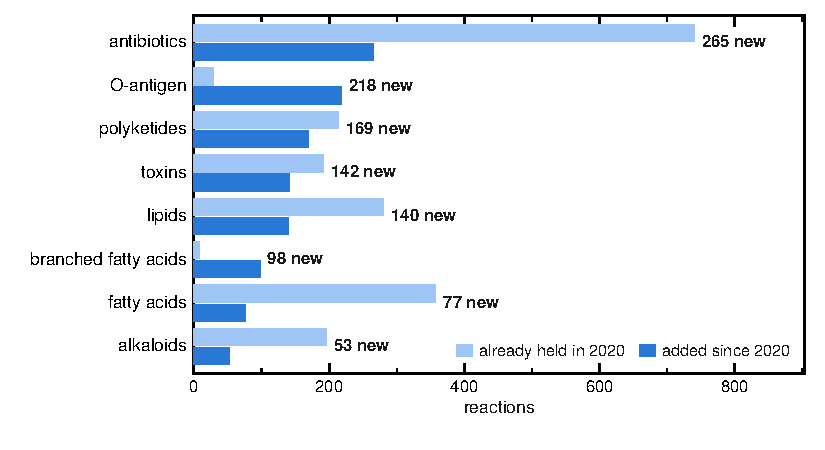
\includegraphics[width=0.85\textwidth]{../figures/figureS1_pathway_classes.pdf}
\caption{\textbf{Where the growth since 2020 landed.} Reactions from MetaCyc that were added since 2020 against those already held. Here we show the eight classes of pathways for which we added the most reactions. Growth is concentrated in specialised metabolism and cell-envelope biosynthesis.}\label{fig:s1} \end{figure}